
\documentclass[tikz,convert={convertexe={magick.exe}}]{standalone}
%\documentclass[tikz,convert]{standalone}
\usetikzlibrary{arrows}

\usepackage{ifthen}

\usepackage{amssymb}
\newcommand{\into}{\mathop{\lrcorner}}

\usetikzlibrary{snakes}
\usetikzlibrary{decorations.pathmorphing}

\begin{document}
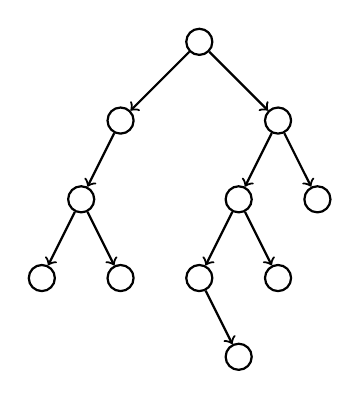
\begin{tikzpicture}[every node/.style={draw=black, circle, thick}, v/.style={->,thick}]

\node (A) at (0,0) {};

\node (B0) at (-1,-1) {};
\node (B1) at (1,-1) {};

\draw[v] (A) -- (B0);
\draw[v] (A) -- (B1);

\node (C0) at (-1.5,-2) {};

\node (C2) at (0.5,-2) {};
\node (C3) at (1.5,-2) {};

\draw[v] (B0) -- (C0);
\draw[v] (B1) -- (C2);
\draw[v] (B1) -- (C3);


\node (D0) at (-2,-3) {};
\node (D1) at (-1,-3) {};
\draw[v] (C0) -- (D0);
\draw[v] (C0) -- (D1);

\node (D2) at (0,-3) {};
\node (D3) at (1,-3) {};

\draw[v] (C2) -- (D2);
\draw[v] (C2) -- (D3);

\node (E) at (0.5, -4) {};
\draw[v] (D2) -- (E);

\end{tikzpicture}
\end{document}